
This Section presents the main results of the eighty experiments performed as defined in Section \ref{subsec:experimental_design}, and the fourty experiments performed in the related work \cite{manfrediReducingReadWrite2024}, conducted with the same experimental desing and environment. The experiments are grouped into subsections according to the measured operation, i.e., read or write. Each Subsection presents histograms and tables to visualize the results using both metrics, i.e., latency (measured in seconds) and throughput (measured in rows/secodns), defined in \gls{RQ}2.

It must be noted that the results are visualized using a log scale for clarity, as results differing from more than one significant figure would not be clearly interpreted using a linear scale, in a histogram representation. For each measurement, a 95\% confidence interval was calculated using the bootstrapping technique mentioned in Section \ref{subsec:method_reliability_validity}. For better readibility, this interval is not reported in the histograms of this Section, but it is reported in Appendices \ref{appx:res_write}--\ref{appx:res_read}, with a histogram and a table for each experiment expressed in both metrics.

Of the two metrics, only latency was measured during the experiments, while throughput was calculated with the formula present in Section ~\ref{subsec:eval_process_hudi_iceberg}. Latency and throughput are inversely related by a constant factor, as all experiments were conducted with fixed-size tables. This implies that halving the latency results in a doubling of throughput, while reducing latency to a quarter results in a quadrupling of throughput. Since the results are described according to both metrics, this introduces redundancy. To minimize repetition, trends will primarily be discussed in terms of latency, with throughput trends highlighted only when they exhibit significantly different behavior.



%%%%%%%%%%%%%%%%%%%%%%%%%%%%%%%%%%%%%%%%%%%%%%%%%%%%%%%%%%%%%%%
%%%%%                  WRITE EXPERIMENTS                  %%%%%
%%%%%%%%%%%%%%%%%%%%%%%%%%%%%%%%%%%%%%%%%%%%%%%%%%%%%%%%%%%%%%%
\subsection{Write experiments}

\begin{figure}
    \centering
    \begin{minipage}[b]{\textwidth}
        \centering
        \captionof{table}[Write experiments results expressed as latency]{Write experiment results expressed as latency. Experiments performed with multiple \glstext{CPU} cores are expressed as latency percentage decrease compared to the one \glstext{CPU} core experiment.}
        \label{tbl:res_write_time_cpu_perc_HID}
        \begin{tabular}{c r S[table-format=4.5] S[table-format=2.2] S[table-format=2.2] S[table-format=2.2]} 
            \toprule
            Pipeline\Tstrut\Bstrut & \thead{Number\\ of rows} & {\thead{1 CPU core latency \\ (seconds)}} & {\thead{2 CPU cores\\ (\% decrease)}} & {\thead{4 CPU cores\\ (\% decrease)}} & {\thead{8 CPU cores\\ (\% decrease)}} \\
            \midrule
            \multirow{5}{4em}{Hudi\\Legacy}             &   10K   &     50.23794  &     -0.98  &     -2.06  &     -1.97  \\
                                                        &  100K   &     59.55605  &     -0.37  &      0.07  &     -1.23  \\
                                                        &    1M   &    112.17773  &      3.22  &      3.00  &      2.49  \\
                                                        &    6M   &    511.84908  &      7.52  &      5.84  &      7.01  \\
                                                        &   60M   &   2716.20939  &     13.81  &     13.63  &     14.41  \\
            \midrule
            \multirow{5}{4em}{Iceberg\\IcedHops}        &   10K   &      1.20406  &      0.75  &      0.73  &     -1.18  \\
                                                        &  100K   &      1.26524  &      5.19  &      0.83  &      1.32  \\
                                                        &    1M   &      1.71770  &     -0.22  &      5.01  &     -0.08  \\
                                                        &    6M   &      3.57649  &      0.28  &      0.88  &      1.23  \\
                                                        &   60M   &     24.60989  &      4.48  &      2.46  &      4.01  \\
            \midrule
            \multirow{5}{4em}{Delta Lake\\delta-rs}     &   10K   &      1.25088  &     -0.95  &      2.72  &     -8.70  \\
                                                        &  100K   &      1.36800  &      4.44  &      2.30  &      5.54  \\
                                                        &    1M   &      9.38231  &      9.19  &     10.27  &     11.59  \\
                                                        &    6M   &     19.75149  &     17.47  &     17.86  &     20.39  \\
                                                        &   60M   &    177.19458  &     24.29  &     29.99  &     31.21  \\
            \bottomrule
        \end{tabular}
    \end{minipage}
    \begin{minipage}[b]{\textwidth}
        \centering
        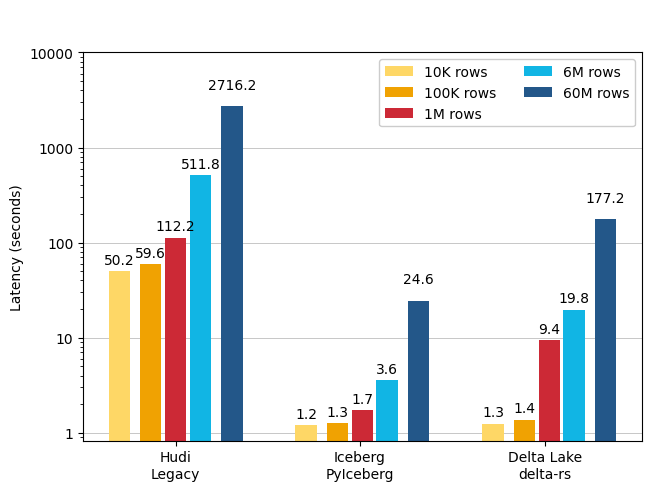
\includegraphics[width=\textwidth]{figures/5-results/hudi_iceberg_delta/write/write_time_1_core.png}
        \caption[Histogram of the write experiment - Latency - 1 CPU core]{Histogram in log-scale of the write experiment results expressed as latency. The experiment was performed with one \glstext{CPU} core.}
        \label{fig:res_write_time_HID}
    \end{minipage}
\end{figure}

\begin{figure}
    \centering
    \begin{minipage}[b]{\textwidth}
        \captionof{table}[Write experiments results expressed as throughput]{Write experiment results expressed as throughput. Experiments performed with multiple \glstext{CPU} cores are expressed as throughput percentage increase compared to the one \glstext{CPU} core experiment.}
        \label{tbl:res_write_throughput_cpu_perc_HID}
        \begin{tabular}{c r S[table-format=4.5] S[table-format=2.2] S[table-format=2.2] S[table-format=2.2]}
            \toprule
            Pipeline\Tstrut\Bstrut & {\thead{Number\\ of rows}} & {\thead{1 CPU core throughput \\ (k rows/second)}} & {\thead{2 CPU cores\\ (\% increase)}} & {\thead{4 CPU cores\\ (\% increase)}} & {\thead{8 CPU cores\\ (\% increase)}} \\
            \midrule
            \multirow{5}{4em}{Hudi\\Legacy}             &   10K   &      0.19905  &     -0.97  &     -2.02  &     -1.93  \\
                                                        &  100K   &      1.67909  &     -0.37  &      0.07  &     -1.21  \\
                                                        &    1M   &      8.91443  &      3.33  &      3.10  &      2.56  \\
                                                        &    6M   &     11.72221  &      8.13  &      6.20  &      7.54  \\
                                                        &   60M   &     22.08961  &     16.02  &     15.78  &     16.84  \\
            \midrule
            \multirow{5}{4em}{Iceberg\\IcedHops}        &   10K   &      8.30521  &      0.75  &      0.74  &     -1.16  \\
                                                        &  100K   &     79.03658  &      5.47  &      0.84  &      1.33  \\
                                                        &    1M   &    582.17295  &     -0.22  &      5.28  &     -0.08  \\
                                                        &    6M   &   1677.62161  &      0.28  &      0.89  &      1.25  \\
                                                        &   60M   &   2438.04452  &      4.69  &      2.52  &      4.18  \\
            \midrule
            \multirow{5}{4em}{Delta Lake\\delta-rs}     &   10K   &      7.99435  &     -0.94  &      2.80  &     -8.00  \\
                                                        &  100K   &     73.09924  &      4.65  &      2.35  &      5.87  \\
                                                        &    1M   &    106.58358  &     10.12  &     11.45  &     13.11  \\
                                                        &    6M   &    303.77453  &     21.16  &     21.75  &     25.61  \\
                                                        &   60M   &    338.61080  &     32.08  &     42.83  &     45.37  \\
            \bottomrule
        \end{tabular}
    \end{minipage}
    \begin{minipage}[b]{\textwidth}
        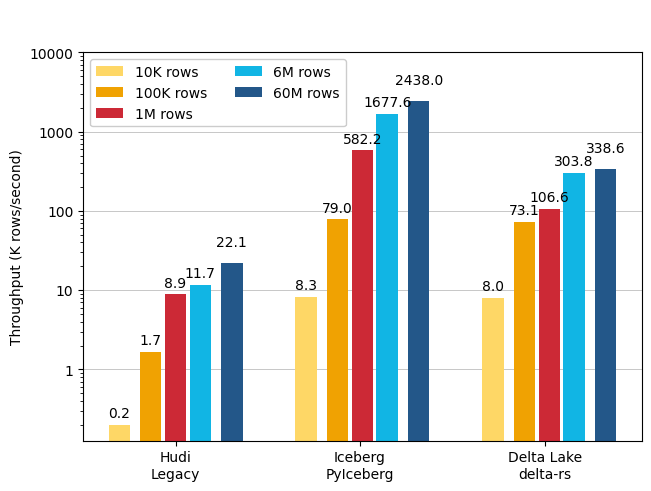
\includegraphics[width=\textwidth]{figures/5-results/hudi_iceberg_delta/write/write_throughput_1_core.png}
        \caption[Histogram of the write experiment - Throughput - 1 CPU core]{Histogram in log-scale of the write experiment results expressed as throughput. The experiment was performed with one \glstext{CPU} core.}
        \label{fig:res_write_throughput_HID}
    \end{minipage}
\end{figure}



Figures~\ref{fig:res_write_time_HID}--\ref{fig:res_write_throughput_HID}, and Tables~\ref{tbl:res_write_time_cpu_perc_HID}--\ref{tbl:res_write_throughput_cpu_perc_HID} report the results of the write experiments performed. The results are expressed in latency in Figure~\ref{fig:res_write_time_HID} and Table~\ref{tbl:res_write_time_cpu_perc_HID}, while are expressed in throughput in Figure~\ref{fig:res_write_throughput_HID} and Table~\ref{tbl:res_write_throughput_cpu_perc_HID}. The experiments were performed on the two systems defined in Section~\ref{subsec:experimental_design} and on the delta-rs based system defined in the related work \cite{manfrediReducingReadWrite2024}. The five tables of different sizes being written were defined in Section~\ref{subsec:experimental_data}.

Both histograms, i.e., Figures~\ref{fig:res_write_time_HID}--\ref{fig:res_write_throughput_HID}, report the results of the experiment performed with one \gls{CPU} core. Instead, Tables~\ref{tbl:res_write_time_cpu_perc_HID}--\ref{tbl:res_write_throughput_cpu_perc_HID} also present a calculated percentage of improvement (decrease in the case of latency, increase in the case of throughput) of the metric as the \gls{CPU} cores increase.

%%%%% WRITE RESULTS /// HUDI vs. ICEDHOPS %%%%%
\subsubsection*{Legacy pipeline vs. IcedHops}
The latency on write operations measured using IcedHops is more than fourty times lower than the latency measured using the legacy pipeline, in all the experiments. This trend is more prominent for bigger tables (6M and 60M rows), where latency measured using IcedHops is less than one hundredth of the latency measured using the legacy system.

%%%%% WRITE RESULTS /// ICEDHOPS vs. DELTA LAKE %%%%%
\subsubsection*{IcedHops vs. delta-rs}
The latency on write operations measured using IcedHops is lower than the latency measured using the delta-rs pipeline, in all the experiments. This trend is more prominent for the biggest table (60M rows), where latency measured using IcedHops is around seven times lower than the latency measured using the delta-rs pipeline, while it is lesser prominent the smaller are the tables, with approximatively equal latency for the smallest table (10K rows).

%%%%% WRITE RESULTS /// PERFORMANCES WITH DIFFERENT CORE(S)
\subsubsection*{Change of performance as the \glsentryshort{CPU} cores increase}
The experiments with increased \gls{CPU} cores showed different results across the different pipeline technologies.  For the legacy system, significant latency reductions were only observed for the largest table (60M rows), with a decrease of approximately 14\%. Smaller tables (10K and 100K rows) actually saw slight increases in latency, and even the larger tables (1M and 6M rows) only improved by a maximum of 7\%. 
IcedHops saw some benefit from additional \gls{CPU} cores, but the improvement was limited, with only a maximum of 5\% descrease in latency for some tables (100K, 60M). 
The most substantial gains were seen with delta-rs, where the larger tables (6M and 60M rows) experienced considerable improvements of 20-30\%, and smaller tables (100K and 1M rows) only saw modest latency decreases of 5-10\%.



%%%%%%%%%%%%%%%%%%%%%%%%%%%%%%%%%%%%%%%%%%%%%%%%%%%%%%%%%%%%%%%
%%%%%                  READ EXPERIMENTS                   %%%%%
%%%%%%%%%%%%%%%%%%%%%%%%%%%%%%%%%%%%%%%%%%%%%%%%%%%%%%%%%%%%%%%
\subsection{Read experiments}

\begin{figure}
    \centering
    \begin{minipage}[b]{\textwidth}
        \captionof{table}[Read experiments results expressed as latency]{Read experiment results expressed as latency. Experiments performed with multiple \glstext{CPU} cores are expressed as latency percentage decrease compared to the one \glstext{CPU} core experiment.}
        \label{tbl:res_read_time_cpu_perc_HID}
        \begin{tabular}{c r S[table-format=4.5] S[table-format=2.2] S[table-format=2.2] S[table-format=2.2]} 
            \toprule
            Pipeline\Tstrut\Bstrut & {\thead{Number\\ of rows}} & {\thead{1 CPU core latency \\ (seconds)}} & {\thead{2 CPU cores\\ (\% decrease)}} & {\thead{4 CPU cores\\ (\% decrease)}} & {\thead{8 CPU cores\\ (\% decrease)}} \\
            \midrule
            \multirow{5}{4em}{Hudi\\Legacy}             &   10K   &      0.63144  &      1.05  &     -0.76  &      0.65  \\
                                                        &  100K   &      2.65043  &     -0.49  &      0.40  &     -0.45  \\
                                                        &    1M   &      8.59296  &     -0.16  &     -1.76  &      2.80  \\
                                                        &    6M   &     33.52580  &      0.44  &      0.23  &      0.26  \\
                                                        &   60M   &     33.69031  &      0.18  &      0.09  &      1.63  \\
            \midrule
            \multirow{5}{4em}{Iceberg\\IcedHops}        &   10K   &      0.01723  &     -6.36  &    -72.94  &      1.53  \\
                                                        &  100K   &      0.04687  &      7.89  &      8.62  &      8.95  \\
                                                        &    1M   &      0.43018  &     37.37  &     45.75  &     46.04  \\
                                                        &    6M   &      2.12331  &     38.96  &     52.50  &     58.34  \\
                                                        &   60M   &     21.81955  &     38.07  &     53.66  &     59.49  \\
            \midrule
            \multirow{5}{4em}{Delta Lake\\delta-rs}     &   10K   &      0.05345  &     22.90  &     18.50  &     19.29  \\
                                                        &  100K   &      0.05763  &      0.73  &      3.78  &      5.18  \\
                                                        &    1M   &      0.53878  &     56.62  &     64.81  &     67.69  \\
                                                        &    6M   &      1.94947  &     53.41  &     72.76  &     74.50  \\
                                                        &   60M   &     22.98186  &     50.35  &     75.72  &     87.19  \\
            \bottomrule
        \end{tabular}
    \end{minipage}
    \begin{minipage}[b]{\textwidth}
        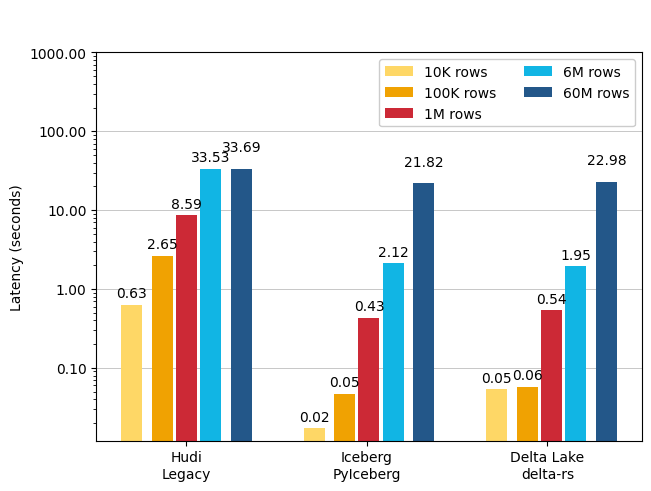
\includegraphics[width=\textwidth]{figures/5-results/hudi_iceberg_delta/read/read_time_1_core.png}
        \caption[Histogram of the read experiment - Latency - 1 CPU core]{Histogram in log-scale of the read experiment results expressed as latency. The experiment was performed with one \glstext{CPU} core.}
        \label{fig:res_read_time_HID}
    \end{minipage}
\end{figure}

\begin{figure}
    \centering
    \begin{minipage}[b]{\textwidth}
        \captionof{table}[Read experiments results expressed as throughput]{Read experiment results expressed as throughput. Experiments performed with multiple \glstext{CPU} cores are expressed as throughput percentage increase compared to the one \glstext{CPU} core experiment.}
        \label{tbl:res_read_throughput_cpu_perc_HID}
        \begin{tabular}{c r S[table-format=4.5] S[table-format=2.2] S[table-format=2.2] S[table-format=2.2]}
            \toprule
            Pipeline\Tstrut\Bstrut & {\thead{Number\\ of rows}} & {\thead{1 CPU core throughput \\ (k rows/second)}} & {\thead{2 CPU cores\\ (\% increase)}} & {\thead{4 CPU cores\\ (\% increase)}} & {\thead{8 CPU cores\\ (\% increase)}} \\
            \midrule
            \multirow{5}{4em}{Hudi\\Legacy}             &   10K   &     15.83673  &      1.06  &     -0.75  &      0.66  \\
                                                        &  100K   &     37.72979  &     -0.48  &      0.40  &     -0.45  \\
                                                        &    1M   &    116.37431  &     -0.16  &     -1.73  &      2.88  \\
                                                        &    6M   &    178.96662  &      0.44  &      0.23  &      0.26  \\
                                                        &   60M   &   1780.92764  &      0.18  &      0.09  &      1.65  \\
            \midrule
            \multirow{5}{4em}{Iceberg\\IcedHops}        &   10K   &    580.48003  &     -5.98  &    -42.18  &      1.56  \\
                                                        &  100K   &   2133.40362  &      8.57  &      9.43  &      9.83  \\
                                                        &    1M   &   2324.62963  &     59.66  &     84.33  &     85.33  \\
                                                        &    6M   &   2825.77691  &     63.83  &    110.53  &    140.02  \\
                                                        &   60M   &   2749.82753  &     61.47  &    115.82  &    146.85  \\
            \midrule
            \multirow{5}{4em}{Delta Lake\\delta-rs}     &   10K   &    187.08171  &     29.70  &     22.69  &     23.89  \\
                                                        &  100K   &   1735.08031  &      0.74  &      3.93  &      5.47  \\
                                                        &    1M   &   1856.03325  &    130.51  &    184.19  &    209.48  \\
                                                        &    6M   &   3077.75801  &    114.64  &    267.09  &    292.19  \\
                                                        &   60M   &   2610.75520  &    101.42  &    311.87  &    680.55  \\
            \bottomrule
        \end{tabular}
    \end{minipage}
    \begin{minipage}[b]{\textwidth}
        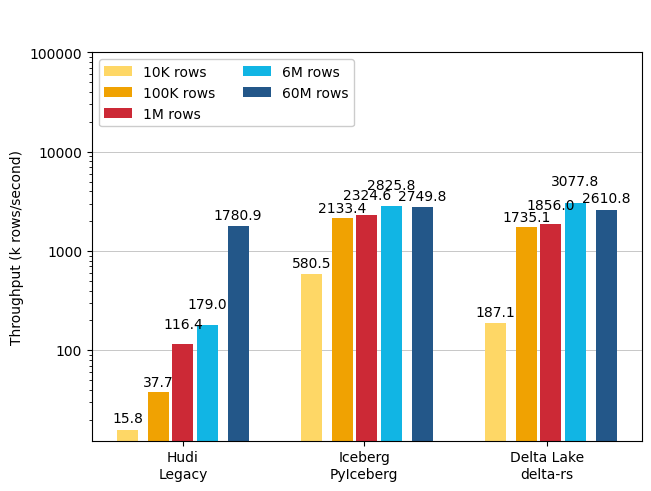
\includegraphics[width=\textwidth]{figures/5-results/hudi_iceberg_delta/read/read_throughput_1_core.png}
        \caption[Histogram of the read experiment - Throughput - 1 CPU core]{Histogram in log-scale of the read experiment results expressed as throughput. The experiment was performed with one \glstext{CPU} core.}
        \label{fig:res_read_throughput_HID}
    \end{minipage}
\end{figure}


Figures~\ref{fig:res_read_time_HID}--\ref{fig:res_read_throughput_HID}, and Tables~\ref{tbl:res_read_time_cpu_perc_HID}--\ref{tbl:res_read_throughput_cpu_perc_HID} report the results of the read experiments performed. The results are expressed in latency in Figure~\ref{fig:res_read_time_HID} and Table~\ref{tbl:res_read_time_cpu_perc_HID}, while are expressed in throughput in Figure~\ref{fig:res_read_throughput_HID} and Table~\ref{tbl:res_read_throughput_cpu_perc_HID}. The experiments were performed on the two systems defined in Section~\ref{subsec:experimental_design} and on the delta-rs based system defined in the related work \cite{manfrediReducingReadWrite2024}. The five tables of different sizes being read were defined in Section~\ref{subsec:experimental_data}.

Both histograms, i.e., Figures~\ref{fig:res_read_time_HID}--\ref{fig:res_read_throughput_HID}, report the results of the experiment performed with one \gls{CPU} core. Instead, Tables~\ref{tbl:res_read_time_cpu_perc_HID}--\ref{tbl:res_read_throughput_cpu_perc_HID} also present a calculated percentage of improvement (decrease in the case of latency, increase in the case of throughput) of the metric as the \gls{CPU} cores increase.

%%%%% READ RESULTS /// HUDI vs. ICEDHOPS %%%%%
\subsubsection*{Legacy pipeline vs. IcedHops}
The latency of read operation measured using IcedHops results from 55\% up to sixty times lower than the latency measured using the legacy pipeline. The most prominent reduction  (sixty times) is obtained in the table containing 100k rows, while the less prominent (55\%) is obtained with the largest table (60M rows). Regarding the other tables, IcedHops has around fifteen times lower read operation latency than the legacy system.

%%%%% READ RESULTS /// ICEDHOPS vs. DELTA LAKE %%%%%
\subsubsection*{IcedHops vs. delta-rs}
The latency on read operations measured using IcedHops is completely comparable with the latency measured using the delta-rs pipeline, if not for the smallest table (10K), where IcedHops latency was three times lower than delta-rs pipeline latency. For the other tables,
The latency on write operations measured using IcedHops is lower than the latency measured using the delta-rs pipeline, in all the experiments. This trend is more prominent for the biggest table (60M rows), where latency measured using IcedHops is around seven times lower than the latency measured using the delta-rs pipeline, while it is lesser prominent the smaller are the tables, with approximatively equal latency for the smallest table (10K rows).

%%%%% READ RESULTS /// PERFORMANCES WITH DIFFERENT CORE(S)
\subsubsection*{Change of performance as the \glsentryshort{CPU} cores increase}
The experiments with increased \gls{CPU} cores showed different results across the different pipeline technologies. In the legacy pipeline, increasing the number of \gls{CPU} cores had minimal impact on latency reduction. The observed improvements remained below 1\% for most table sizes, with some cases even showing slight increases.
IcedHops saw some benefit from utilizing multiple \gls{CPU} cores. While the smallest table (10K rows) showed a slight increase in latency, all other tables benefited from latency reductions. For tables larger than 100K rows, the reduction was more pronounced, reaching around 39\% for mid-sized and large tables (1M, 6M, and 60M rows).
Delta-rs showed the most substantial gains in read latency with additional CPU cores. For small tables (10K and 100K rows), the letancy reductions remained below 5\%, but for tables larger than 100K rows, the reduction was significant, reaching around 55\% for mid-sized table (1M rows) and around 50\% for larger tables (6M and 60M rows).
The trend continued with additional cores, further enhancing performance as table sizes increased.



%%%%%%%%%%%%%%%%%%%%%%%%%%%%%%%%%%%%%%%%%%%%%%%%%%%%%%%%%%%%%%%
%%%%%                  LEGACY BREAKDOWN                   %%%%%
%%%%%%%%%%%%%%%%%%%%%%%%%%%%%%%%%%%%%%%%%%%%%%%%%%%%%%%%%%%%%%%
\subsection{Legacy pipeline write latency breakdown}
\begin{figure}
    \centering
    \begin{minipage}[b]{\textwidth}
        \captionof{table}[Writes on legacy pipeline - Time breakdown]{Contributions to the write latency of the upload and materialization steps in the legacy pipeline. Experiments performed with multiple \glstext{CPU} cores are expressed as latency percentage decrease compared to the one \glstext{CPU} core experiment.}
        \label{tbl:hudi_virtualiz_breakdown_cpu_perc}
        \begin{tabular}{r S[table-format=4.2] S[table-format=4.2] S[table-format=2.2] S[table-format=2.2] S[table-format=2.2] S[table-format=2.2] S[table-format=2.2] S[table-format=2.2]} 
            \toprule
            \multirow{2}{*}{{\thead{Number\\ of rows}}} & \multicolumn{2}{c}{{\thead{1 CPU core\\ latency (seconds)}}} & \multicolumn{2}{c}{{\thead{2 CPU cores\\ (\% decrease)}}} & \multicolumn{2}{c}{{\thead{4 CPU cores\\ (\% decrease)}}} & \multicolumn{2}{c}{{\thead{8 CPU cores\\ (\% decrease)}}}\\
            & {upl.} & {mat.} & {upl.} & {mat.} & {upl.} & {mat.} & {upl.} & {mat.}\\
            \midrule
            10K &  2.50 & 47.73 & 4.50 & -1.28 & 4.53 & -2.46 & 4.65 & -2.32\\
            100K & 3.67 & 55.91 & 6.36 & -0.79 & 5.56 & -0.30 & 6.28 & -1.68\\
            1M   & 22.59 & 89.60 & 17.51 & -0.37 & 14.88 & 0.01 & 16.49 & -1.03\\
            6M   & 244.60 & 267.25 & 15.83 & -0.10 & 13.47 & -1.15 & 15.09 & -0.39\\
            60M &  2438.22 & 278.16 & 15.34 & 0.43 & 15.17 & 0.20 & 15.96 & 0.86\\
            \bottomrule
        \end{tabular}
    \end{minipage}
    \begin{minipage}[b]{\textwidth}
        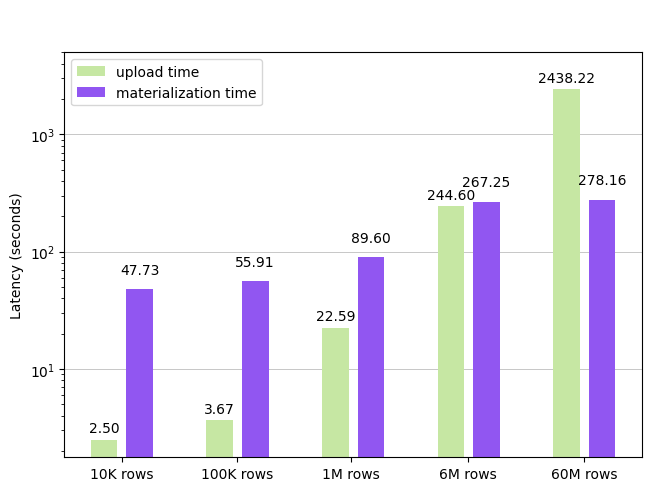
\includegraphics[width=\textwidth]{figures/5-results/hudi_iceberg_delta/hudi_virtualiz1_core.png}
        \caption[Histogram of the write on legacy pipeline - Time breakdown - 1 core]{Histogram in log-scale displaying the contributions to the write latency of the upload and materialization steps in the legacy pipeline. The experiment was performed with one \glstext{CPU} core.}
        \label{fig:hudi_virtualiz_breakdown}
    \end{minipage}
\end{figure}

Table \ref{tbl:hudi_virtualiz_breakdown_cpu_perc} and Figure \ref{fig:hudi_virtualiz_breakdown} show the write latency breakdown of the legacy pipeline into upload time and materialization time, the two different steps explained in Section \ref{subsec:back_sys_hudi_write}. The breakdown is proposed for all five tables defined in Section \ref{subsec:experimental_data}. Figure \ref{fig:hudi_virtualiz_breakdown} reports the data from the one \gls{CPU} core experiment. In contrast, Table \ref{tbl:hudi_virtualiz_breakdown_cpu_perc} reports both the one \gls{CPU} core experiment data and also a calculated percentage of improvement (decrease) of the latency as the \gls{CPU} cores increase.

Considering the upload time contribution to the write latency, this represents a small percentage (around 5\%) when writing smaller tables (10K and 100K) rows, while it grows following a similarly linear pattern in larger tables (100K, 6M, and 60M rows). This radically changes the proportion between the upload and materialized time contributions, making the upload time 90\% of the total write latency for the largest table (60M rows). Differently, the materialization time contribution makes up 95\% of the total write latency for the smallest table (10K rows), but then its absolute value does not increase by more than a significant figure even if the table size is increased by three significant figures.

Analyzing the impact of multiple \gls{CPU} cores, the upload time benefits significantly from increased core availability, particularly for larger tables, where latency decreases by 15\% compared to just 4\% for smaller tables. In contrast, the materialize time remains largely unaffected, showing only minor fluctuations, with latency varying by 1-2\%.



%%%%%%%%%%%%%%%%%%%%%%%%%%%%%%%%%%%%%%%%%%%%%%%%%%%%%%%%%%%%%%%
%%%%%                   IN-MEMORY USAGE                   %%%%%
%%%%%%%%%%%%%%%%%%%%%%%%%%%%%%%%%%%%%%%%%%%%%%%%%%%%%%%%%%%%%%% 
\subsection{In-memory resources usage}
\label{subsec:resources_usage}

The resources of the experimental environment, defined in Section \ref{subsec:experimental_env}, were adjusted to match computational needs. The write operations were demanding on the available \gls{RAM} resources, requiring up to 24 GBs to operate with the larger tables (6M and 60M rows). Thus, on were allocated 32768 MBs of \gls{RAM}, to avoid slowing down operations.